\section{Praktische Analyse}


\subsection{Programmierfehler}
Grundsätzlich kann jede Software von Buffer Overflows betroffen sein, die in einer Programmiersprache geschrieben ist,
welche direkte Zugriffe auf die Speicherstrukturen des Systems ermöglicht. Beispiele hierfür wären: Assembler, C/C++ oder
Fortran. Prinzipiell nicht betroffen sind Programme, die in einer interpretierten Sprache wie Python oder Java geschrieben
sind. Bei diesen Sprachen wäre nur ein Overflow im Interpreter selber möglich, da dieser in der Regel auf einer der zuerst
genannten Sprachen basiert.

Am problematischsten sind hierbei Funktionen, die es ermöglichen Nutzereingaben zu lesen und zu speichern,
die jedoch nicht die Länge der eingegebenen Daten überprüfen können. Zwei der bekanntesten Vertreter für Funktionen
dieser Art sind die C Funktionen \codeline{gets()} und \codeline{strcopy()}:
\begin{itemize}
    \item \codeline{gets(buffer)} Fragt nach Input und kopiert die Eingaben in den angegebenen Speicher
    \item \codeline{strcopy(buffer, input)} Kopiert den Input (z.\,B. ein Kommandozeilenargument)\\ in den angegebenen Speicher
\end{itemize}
Da keine Kontrolle auf die Länge des Inputs durchgeführt wird, kann nicht sichergestellt werden,
dass der angegebene Speicherbereich ausreichend groß ist oder ob der Input in andere Bereiche überläuft.

\subsection{Format-String-Schwachstelle}
Bei Format-String-Schwachstellen handelt es sich zwar nicht direkt um eine Art von Buffer Overflow,
jedoch können diese oft in ähnlichen Kontexten aufkommen und ermöglichen es Angreifern,
Informationen über die Interna eines Programms zu gewinnen.

Problematisch ist hierbei die unvorsichtige Verwendung von Formatierungsfunktionen wie \codeline{fprint()}.
Soll beispielsweise eine Zeichenkette ausgegeben werden, sollte korrekterweise ein Formatierungsparameter
wie \codeline{\%s} verwendet werden: \codeline{printf(“\%s”, chars)}. Die Unterschlagung dieses Parameters
scheint zwar auf den ersten Blick dasselbe Ergebnis zu liefern: \codeline{printf(chars)}. Die zweite Variante ermöglicht
es dem Angreifer jedoch, eigene Parameter einzusetzen, um Informationen auszulesen oder zu manipulieren:
\begin{itemize}
    \item \codeline{\%x} Liest Daten vom Stack
    \item \codeline{\%s} Liest Strings aus dem Prozess
    \item \codeline{\%n} Schreibt einen Integer in den Prozess
    \item \codeline{\%p} Gibt Pointer auf void aus
\end{itemize}
\pagebreak %MUSS WEG BEI ÄNDERUNG

\subsection{Szenario}
Im Folgenden wird nun ein konstruiertes Szenario in einer virtuellen Umgebung betrachtet.
Die beiden Akteure sind auf der einen Seite ein Linux Server, der eine verwundbare C-Applikation über einen Port
bereitstellt, und auf der anderen Seite eine Kali Box, die die Rolle des Angreifers übernimmt.

Es wird davon ausgegangen, dass der Angreifer mindestens über eine Kopie der Software verfügt. Für einen Angriff
ist dies zwar prinzipiell nicht notwendig, jedoch ermöglicht es ihm eine detailliertere Analyse der Software in
einer Debugging-Umgebung.
\subsection{C-Programm}
Das bereitgestellte C-Programm springt aus \codeline{main()} in eine Funktion \codeline{gruss()}.
Hier wird ein Char Array mit einer Größe von 256 Bytes auf dem Stack angelegt und der Nutzer mit der \codeline{gets()} Funktion
nach seinem Namen gefragt. Dieser wird anschließend mit der iterate Funktion von vorne nach hinten durchiteriert
und anschließend mit \codeline{printf()} ausgegeben. Die Funktion wird dann in einer Schleife immer wieder aufgerufen.

\begin{figure}[h]
    \centering
    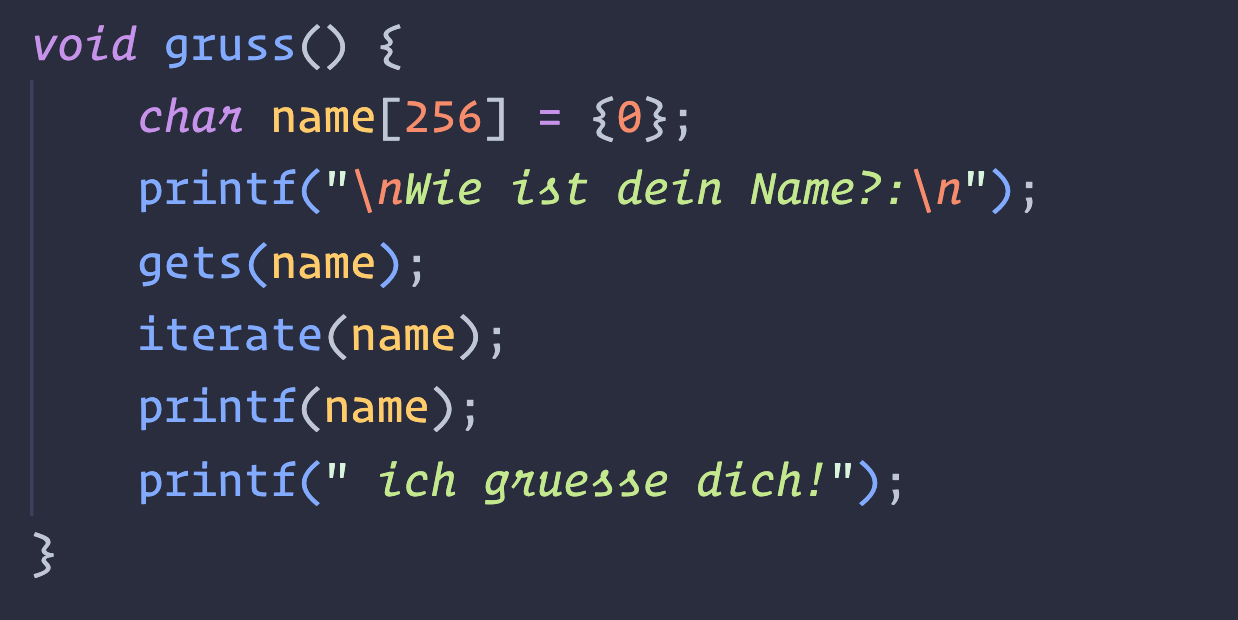
\includegraphics[width=0.6\textwidth,height=0.75\textheight,keepaspectratio]{images/gruss.png}
    \caption{Funktion \codeline{gruss()}}
\end{figure}
Mit einem Blick in den Source Code und durch einige Test-Eingaben lässt sich schnell erkennen,
dass Namen mit einer großen Länge zu einem Absturz bzw. zu einem Segmentation Fault führen.

\begin{figure}[h]
    \centering
    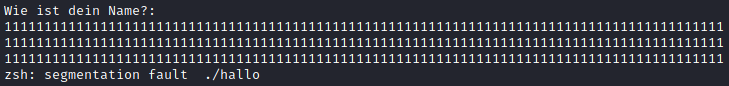
\includegraphics[width=0.8\textwidth,height=0.75\textheight,keepaspectratio]{images/segfault.png}
    \caption{Segmentierungsfehler}
\end{figure}

Außerdem können durch Eingabe von Formatierungsparametern Informationen, wie Speicheradressen, ausgeben werden.

\begin{figure}[h]
    \centering
    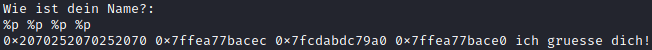
\includegraphics[width=0.8\textwidth,height=0.75\textheight,keepaspectratio]{images/adressen.png}
    \caption{Ausgegebene Speicheradressen}
\end{figure}

Das Programm weist also eine Stack basierte Buffer-Overflow- und eine Format-String-Schwachstelle auf.

\subsection{Debugging}

Um diese Schwachstellen nun jedoch gezielt auszunutzen und Shellcode in den Prozess zu injizieren,
muss dieser zunächst in einem Debugger analysiert werden. Wegen seines simplen, aber funktionalen Aufbaus
fällt die Wahl auf den GNU Debugger.

Ein Blick in die Memory Map des laufenden Prozesses zeigt, dass die zweite Adresse der Format-String-Ausgabe
in den Stack verweist.
\begin{figure}[h]
    \centering
    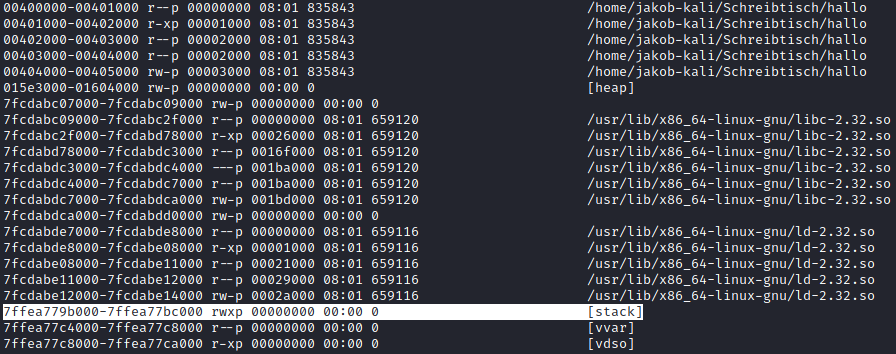
\includegraphics[width=0.9\textwidth,height=0.75\textheight,keepaspectratio]{images/map.png}
    \caption{Memory Map}
\end{figure}

Mit dem Wissen, worauf diese Adresse verweist, lassen sich andere Adressen relativ zu dieser berechnen und
ASLR (Address Space Layout Randomization) umgehen.

Der GDB wird nun an den Prozess angehängt und ein Breakpoint an das Ende der \codeline{gruss()} Funktion gesetzt.
In das Programm werden nun einige leicht wiedererkennbare Zeichenketten eingegeben und der Speicher um die
betrachtete Adresse untersucht. Dabei fällt auf, dass sich die Adresse je nach Länge der Eingabe verschiebt.
Aus den Beobachtungen lässt sich schließen, dass die Adresse immer auf das Ende der Eingabe im Buffer zeigt.
\begin{figure}[h]
    \centering
    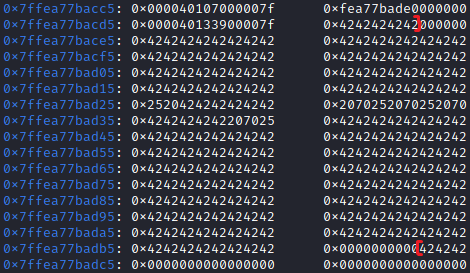
\includegraphics[width=0.6\textwidth,height=0.75\textheight,keepaspectratio]{images/buffer.png}
    \caption{Speicherinhalt}
    \label{fig:spinhalt}
\end{figure}

(Die roten Klammern in \autoref{fig:spinhalt} markieren den Anfang und das Ende der Eingabe)

Um die Adresse des Instruction Pointers herauszufinden, generieren wir uns eine möglichst zufällige,
lange Zeichenkette und geben sie in das Programm ein. Der darauf folgende Segmentation Fault lässt vermuten,
dass der Instruction Pointer überschrieben wurde und nun auf eine ungültige Adresse zeigt. Im Debugger lassen wir
uns den Inhalt des RIP-Registers ausgeben und suchen ihn in unserer generierten Zeichenkette. Wenn wir diesen und
alle folgenden Zeichen jetzt aus unserer Kette löschen, so bleiben noch 264 Zeichen. Wir wissen also: Wenn wir unseren
Buffer mit 264 Zeichen füllen, sind die darauf folgenden 8 Bytes der gesuchte Instruction Pointer.

\subsection{Exploit} \label{sec:explainersub}
Mit diesem Wissen kann nun ein Exploit für das C-Programm geschrieben werden, mit dessen Hilfe beliebiger Shellcode
auf dem Zielsystem ausgeführt werden kann. Hierfür muss zunächst ein Payload-Aufbau gewählt werden:
\begin{enumerate}
    \item An das Programm werden 264 Zeichen, gefolgt von einem konstruierten RIP, gegeben, der auf den nachfolgenden Shellcode zeigt
\end{enumerate}
\begin{figure}[h]
    \centering
    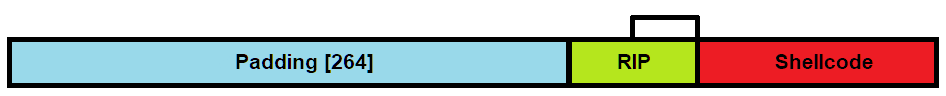
\includegraphics[width=0.8\textwidth,height=0.75\textheight,keepaspectratio]{images/payload1.png}
    \caption{Payload 1}
\end{figure}

\begin{enumerate}
    \setcounter{enumi}{1}
    \item Der Shellcode wird mit in den Buffer geschrieben, der RIP zeigt dann in den Buffer
\end{enumerate}
\begin{figure}[h]
    \centering
    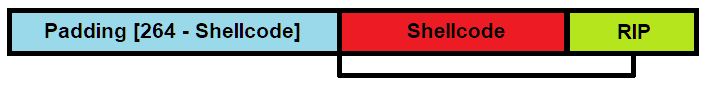
\includegraphics[width=0.8\textwidth,height=0.75\textheight,keepaspectratio]{images/payload2.png}
    \caption{Payload 2}
\end{figure}

Je nach Größe des Buffers/Shellcode und der vorhandenen Abwehrmechanismen kann die eine oder die andere Variante besser sein.
Um Ungenauigkeiten auszugleichen, können zusätzlich noch NOP Slides zum Einsatz kommen. Hierbei handelt es sich um eine Folge
von NOP (0x90) Anweisungen, in deren Mitte dann ungefähr mit dem RIP gezeigt wird.
\begin{figure}[h]
    \centering
    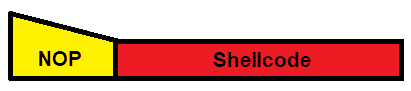
\includegraphics[width=0.5\textwidth,height=0.75\textheight,keepaspectratio]{images/nop.png}
    \caption{NOP Slide}
\end{figure}

Die NOPs fungieren dann als eine Art “Rutsche“ (Slide), an der entlang das Programm an den Anfang des
Shellcodes geführt wird.

\pagebreak

Im folgenden Beispiel-Exploit wählen wir die erste Variante und verwenden zusätzlich eine NOP Slide:
\begin{enumerate}
    \item Nach einem erfolgreichen Verbindungsaufbau senden wir dem Dienst eine Folge von Format-String-Parametern, um uns die Startadresse des Buffers zu berechnen:
\end{enumerate}
\begin{figure}[h]
    \centering
    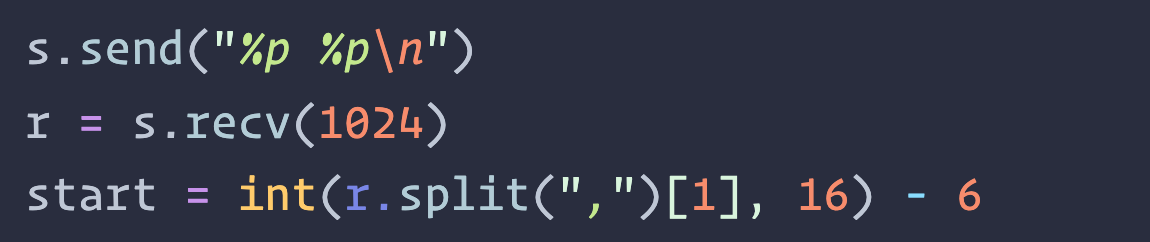
\includegraphics[width=0.6\textwidth,height=0.75\textheight,keepaspectratio]{images/format.png}
    \caption{Format-String-Ausgabe}
\end{figure}

\begin{enumerate}
    \setcounter{enumi}{1}
    \item Mit der Startadresse und unseren 264 Zeichen können wir jetzt den RIP berechnen. Dabei addieren wir noch 16 auf unseren RIP, um in die Mitte der NOP Slide zu zeigen:
\end{enumerate}
\begin{figure}[h]
    \centering
    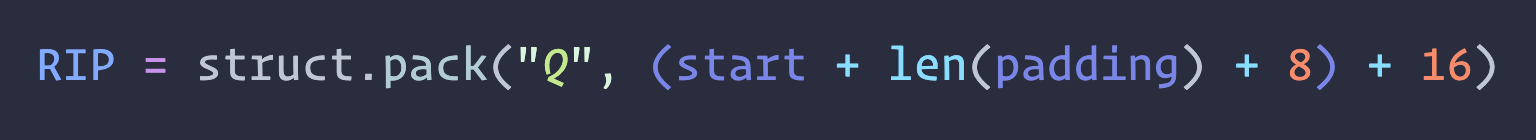
\includegraphics[width=0.8\textwidth,keepaspectratio]{images/rip.png}
    \caption{RIP}
\end{figure}

\begin{enumerate}
    \setcounter{enumi}{1}
    \item Die finale Payload setzt sich dann aus Padding, RIP, NOP Slide und Shellcode zusammen:
\end{enumerate}
\begin{figure}[h]
    \centering
    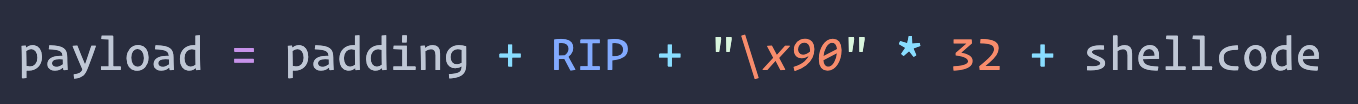
\includegraphics[width=0.8\textwidth,keepaspectratio]{images/payload.png}
    \caption{Payload}
\end{figure}

Nach dem Ausführen des Exploits wird aus dem Prozess eine Shell geöffnet, mit der wir interagieren können.
\begin{figure}[b!]
    \centering
    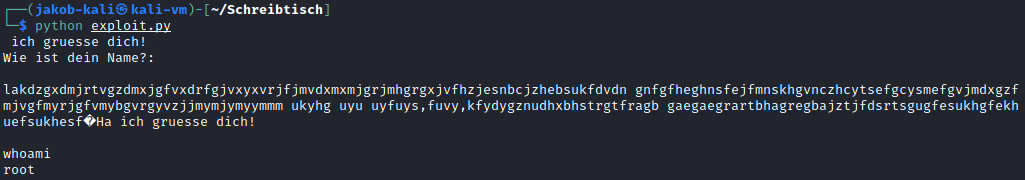
\includegraphics[width=0.9\textwidth,keepaspectratio]{images/root.png}
    \caption{Root Shell}
\end{figure}
Unsere Berechtigungen entsprechen dabei denen des Prozesses: